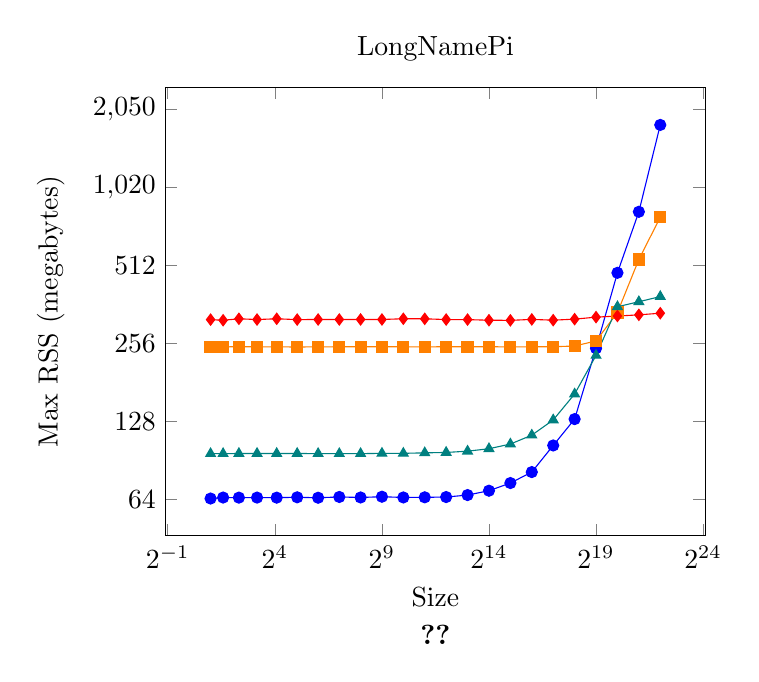
\begin{tikzpicture}
\begin{axis}
[title=LongNamePi,
xlabel={Size},
ylabel={Max RSS (megabytes)},
legend to name=legend,
legend columns=2,
xmode=log,
log basis x={2},
ymode=log,
log basis y={2},
yticklabel={
  \pgfkeys{/pgf/fpu=true}
  \pgfmathparse{pow(2,\tick)}
  \pgfmathprintnumber[fixed relative,precision=3]{\pgfmathresult}
  \pgfkeys{/pgf/fpu=false}
}]
\addplot [
color=blue,
mark=o,
only marks,
forget plot
] coordinates {

};
\addplot [
color=orange,
mark=square,
only marks,
forget plot
] coordinates {

};
\addplot [
color=red,
mark=diamond,
only marks,
forget plot
] coordinates {

};
\addplot [
color=teal,
mark=triangle,
only marks,
forget plot
] coordinates {

};
\addplot [
color=blue,
mark=*
] coordinates {
(4194305.0,1787.53536) 
(2097153.0,826.085376) 
(1048577.0,480.227328) 
(524289.0,245.485568) 
(262145.0,130.863104) 
(131073.0,103.542784) 
(65537.0,81.727488) 
(32769.0,74.153984) 
(16385.0,69.267456) 
(8193.0,66.637824) 
(4097.0,65.470464) 
(2049.0,65.314816) 
(1025.0,65.236992) 
(513.0,65.662976) 
(257.0,65.224704) 
(129.0,65.519616) 
(65.0,65.069056) 
(33.0,65.323008) 
(17.0,65.1264) 
(9.0,65.163264) 
(5.0,65.134592) 
(3.0,65.183744) 
(2.0,64.6144) 
};
\addlegendentry{Agda}
\addplot [
color=orange,
mark=square*
] coordinates {
(4194305.0,787.116032) 
(2097153.0,540.921856) 
(1048577.0,337.563648) 
(524289.0,262.127616) 
(262145.0,250.580992) 
(131073.0,248.950784) 
(65537.0,248.860672) 
(32769.0,248.664064) 
(16385.0,248.942592) 
(8193.0,248.827904) 
(4097.0,248.860672) 
(2049.0,248.782848) 
(1025.0,248.786944) 
(513.0,248.909824) 
(257.0,248.91392) 
(129.0,248.897536) 
(65.0,248.659968) 
(33.0,248.406016) 
(17.0,248.672256) 
(9.0,248.836096) 
(5.0,248.946688) 
(3.0,248.745984) 
(2.0,248.926208) 
};
\addlegendentry{Idris 2}
\addplot [
color=red,
mark=diamond*
] coordinates {
(4194305.0,335.429632) 
(2097153.0,330.514432) 
(1048577.0,327.139328) 
(524289.0,323.854336) 
(262145.0,318.173184) 
(131073.0,315.273216) 
(65537.0,317.41952) 
(32769.0,314.806272) 
(16385.0,315.109376) 
(8193.0,316.870656) 
(4097.0,317.018112) 
(2049.0,319.123456) 
(1025.0,319.295488) 
(513.0,317.198336) 
(257.0,317.247488) 
(129.0,317.21472) 
(65.0,317.206528) 
(33.0,316.862464) 
(17.0,319.209472) 
(9.0,317.059072) 
(5.0,319.205376) 
(3.0,314.9824) 
(2.0,316.788736) 
};
\addlegendentry{Lean 4}
\addplot [
color=teal,
mark=triangle*
] coordinates {
(4194305.0,388.866048) 
(2097153.0,371.429376) 
(1048577.0,355.229696) 
(524289.0,230.477824) 
(262145.0,163.545088) 
(131073.0,129.88416) 
(65537.0,113.475584) 
(32769.0,104.83712) 
(16385.0,100.589568) 
(8193.0,98.4064) 
(4097.0,97.308672) 
(2049.0,96.964608) 
(1025.0,96.555008) 
(513.0,96.538624) 
(257.0,96.284672) 
(129.0,96.264192) 
(65.0,96.313344) 
(33.0,96.39936) 
(17.0,96.382976) 
(9.0,96.415744) 
(5.0,96.387072) 
(3.0,96.288768) 
(2.0,96.256) 
};
\addlegendentry{Rocq}
\end{axis}
\node[anchor=north] at (current axis.below south) {\ref{legend}};
\end{tikzpicture}
